% mainfile: ../../../../master.tex
\subsection{Comparison of nucleic acid amount obtained with either MasterPure\texttrademark~ or AllPrep kits}
% The part of the label after the colon must match the file name. Otherwise,
% conditional compilation based on task labels does NOT work.
\label{task:20180220_cj0}
\tags{r,qnt,dna,rna}
\authors{cj}
%\files{}
%\persons{}

I have a meeting tomorrow with Viggó and I would like to show my results, especially the results of my DNA/RNA extractions with the MasterPure\texttrademark~ and AllPrep kits. 

% Listing
\begin{lstlisting}[language=r, caption=Comparison of nucleic acid amounts measured by fluorometric-based assay, label=lst:20180220_comparison_qnt]
# load library for plotting
library(ggplot2)

# set up the date to keep files organised
today <- "20180220"

# set the directory to save img
img.path="/Users/Clara/Projects/diary/graphics/plots/"
file.path="/Users/Clara/Projects/mime/res/"

# import colours
source("/Users/Clara/Projects/colors/colors.R")
source("/Users/Clara/Projects/colors/colors2.R")

# enter data
# here I build the dataframe from scratch
values <- c(3.11, 2.44, 5.86, 18.2, 
	7.20, 8.77, 31.5, 32.2,
	25.7, 4.10, 4.10, 95.7,
	15.7, 15.0, 35.1, 48.0)

methods <- c("qubit.dna.br", "qubit.dna.br", "qubit.dna.br", "qubit.dna.br",
	"qubit.rna.br", "qubit.rna.br", "qubit.rna.br", "qubit.rna.br",
	"nanodrop.dna", "nanodrop.dna", "nanodrop.dna", "nanodrop.dna",
	"nanodrop.rna", "nanodrop.rna", "nanodrop.rna", "nanodrop.rna")

kits <- c('MasterPure','AllPrep','AllPrep', "MasterPure",
 	'MasterPure','AllPrep','AllPrep', "MasterPure",
 	'MasterPure','AllPrep','AllPrep', "MasterPure",
 	'MasterPure','AllPrep','AllPrep', "MasterPure")

volumes.ul <- c(50, 100, 150, 50,
	50, 50, 80, 50,
	50, 100, 150, 50,
	50, 50, 80, 50)

labels <- c('MasterPure 1','AllPrep 1','AllPrep 2', "MasterPure 2",
 	'MasterPure 1','AllPrep 1','AllPrep 2', "MasterPure 2",
 	'MasterPure 1','AllPrep 1','AllPrep 2', "MasterPure 2",
 	'MasterPure 1','AllPrep 1','AllPrep 2', "MasterPure 2")

nucl.ac <- data.frame(labels, kits, methods, values, volumes.ul)

nucl.ac$total.ng <- nucl.ac$values * nucl.ac$volumes.ul

# create a minimalist theme for the plot
my.theme <- theme_void() + theme(
	text = element_text(colour=DarkGrey),
	axis.title = element_text(colour=DarkGrey),
	axis.text = element_text(colour=DarkGrey),
	panel.grid.major.y = element_line(colour = LightGrey))

# plot the results
pdf(file = paste(img.path, today, "_nucleic_acid_amount.pdf", sep="", collapse=NULL), 
	width=8, height=4)
ggplot(nucl.ac[nucl.ac$methods!="nanodrop.dna" & nucl.ac$methods!="nanodrop.rna",], 
	aes(labels, total.ng, fill=methods)) +
	geom_col(position="dodge",width=0.5) +
	scale_fill_manual("Fluorometric\nquantification\nmethod", values=c(Carrot,Aqua), 
		labels=c("Qubit dsDNA BR","Qubit RNA BR")) +
	my.theme +
	labs(#title = "Comparison of nucleic acid amounts", 
		#subtitle = "DNA and RNA simultaneous extraction from micro-algae cultures with MasterPure or AllPrep kits",
		x = "Extraction method",
		y = "Nucleic acid amount (ng \ uL)"
		)
dev.off()
\end{lstlisting}

% 


\begin{figure}[H] % position of the figure 
    \centering
    \caption{Comparison of nucleic acid amounts obtained with MasterPure\texttrademark~ and AllPrep kits}
    \label{fig:20180220_nucleic_acid_amount}
    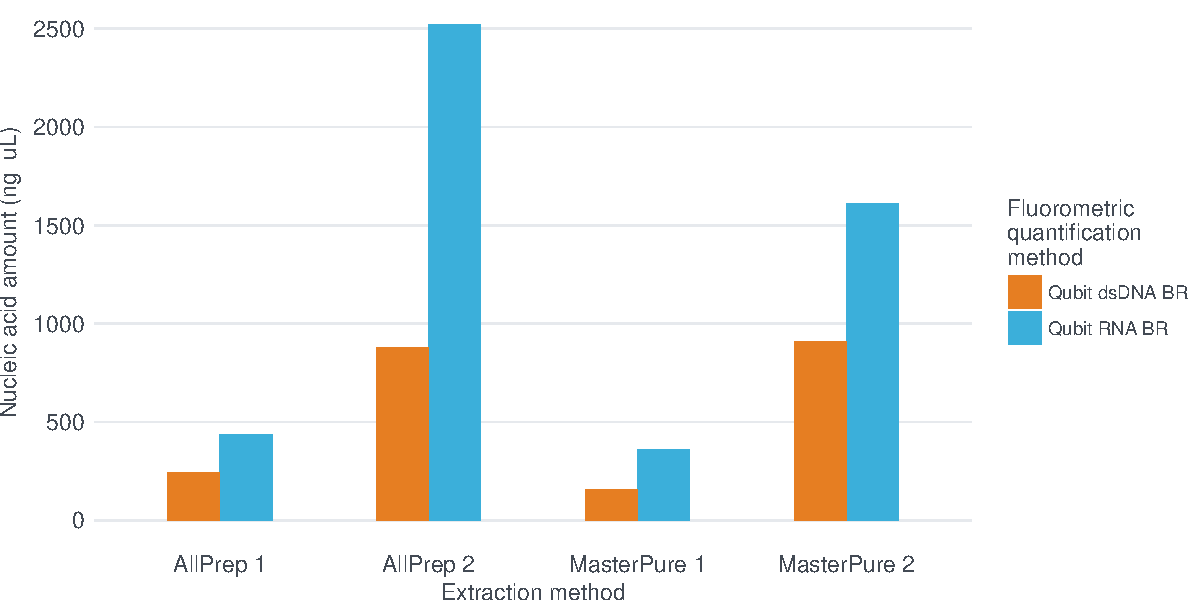
\includegraphics[width=\textwidth]{graphics/plots/20180220_nucleic_acid_amount.pdf}
\end{figure}